\chapter{A look to the future}
\label{chap:future}

\section{Current limitations and the future of non-asymptotic metrology}

Non-asymptotic quantum metrology, as we have defined it in this thesis, was born out of the necessity of applying metrology techniques to situations with a limited amount of experimental data and a potentially moderate amount of prior knowledge, both of which generally lie outside of the scope of the theory based on the Fisher information and the Cram\'{e}r-Rao bound. At the heart of our approach lies the idea of developing an alternative way of doing quantum metrology by relying less on formal approximations and more on the identification of the physically relevant quantities. Nevertheless, our methodology is only the first iteration towards the completion of this task, and despite the wealth of new results that we have uncovered using our formalism, there are still potentially important upgrades for our methods.

One of the crucial tasks that we identified in chapters \ref{chap:limited} and \ref{chap:multibayes} as a potential upgrade is to extend our methods to cover experiments that not only operate in the regime of limited data, but that are also affected by the presence of noise. In the next section we will carry out a first simple analysis of an optical scheme with photon losses, and we will highlight important features to be explored in future work when these two realistic effects are taken into account in a combined fashion. 

Another interesting possibility for future work would be to implement in the laboratory those schemes that have been optimised using our shot-by-shot approach in chapters \ref{chap:limited} and \ref{chap:multibayes}. Let us illustrate how we would proceed with a single-parameter example. Given an experimental arrangement whose information is summarised in the quantum probability $p(m|\theta) = \mathrm{Tr}[E(m) \rho(\theta)]$, and given a moderate amount of prior knowledge encoded in $p(\theta)$, the first step is to find the optimal single-shot strategy that reaches the minimum of the square error $\bar{\epsilon}_{\mathrm{mse}} = \int d\theta dm\hspace{0.15em} p(\theta) p(m|\theta) [g(m) - \theta]^2$, which can be achieved by means of the single-shot quantum optimisation reviewed and exploited in chapter \ref{chap:limited} and in sections \ref{subsec:singleshotparadigm}, \ref{subsec:originalderivation} and \ref{loss}. This process will provide us with either the optimal POM $E(m) \equiv e_m^\mathrm{opt}$ for a given state, the optimal state $\rho_0^\mathrm{opt}$ for a given measurement, or a state and measurement that are both optimal. Although this is the same step that initiated our theoretical study of chapter \ref{chap:limited}, it is also the point where theory and experiment diverge. Our aim was to study the fundamental behaviour of schemes that operate with a limited amount of data, and as such the uncertainty that we have calculated has been averaged over both the parameter and the measurement outcomes. However, in a real-world experiment we will have a concrete string of outcomes, and according to our discussion in section \ref{sec:uncertainty}, the experimental error needs to be based on a figure of merit that depends on such outcomes, that is, in equation (\ref{errexp}) after having chosen the square error. Whether we know how to implement $e^\mathrm{opt}_m$ or how to prepare $\rho_0^\mathrm{opt}$ is a question beyond the scope of our method, although we note that our study with genetic algorithms in section \ref{sec:genetic} demonstrates that the shot-by-shot strategy may be made feasible with current technology. 

It is also important to note that the amount of resources per trial, given by $\langle R \rangle$ with resource operator $R$ (section \ref{sec:problem}), has been assumed to be small. While this assumption guarantees that our results are relevant for and applicable to sensing fragile systems \cite{eckert2007, pototschnig2011, carlton2010, taylor2013, taylor2015, taylor2016, PaulProctor2016}, it excludes other applications where a still finite but larger number of resources per trial may be allowed even if the data is still limited. As we saw in chapter \ref{chap:intro}, this is the case, in particular, for remote sensing \cite{shabir2015, kebei2013, lanzagorta2012, wang2016,zhuang2017}. Fortunately, increasing $\langle R \rangle$ does not alter the foundations of our methodology, and our methods can also be applied in those cases by simply using matrices with larger dimensions for the numerical simulation of the physical system under consideration. 

In terms of theoretical progress, our hybrid method based on selecting the optimal estimator and the asymptotically optimal quantum strategy opens the door to revisiting quantum metrology protocols that have been optimised using the Fisher information and the Cram\'{e}r-Rao bound, which are the majority. More concretely, we could perform a non-asymptotic analysis such as those in chapters \ref{chap:nonasymptotic} and \ref{chap:networks} to determine which of the results found by other authors in the context of the asymptotic theory could be carried over to and exploited in the non-asymptotic regime. 

Importantly, the hybrid method relies on the existence of an asymptotic approximation that coincides with the quantum Cram\'{e}r-Rao bound. A weaker possibility would be returning to $\int d\boldsymbol{\theta}p(\boldsymbol{\theta})F(\boldsymbol{\theta})^{-1}/\mu$ as a more general approximation for the matrix error $\Sigma_{\mathrm{mse}}$, and attempting to use such expression as a guide to select the quantum strategy by comparing different protocols, provided that $F(\boldsymbol{\theta})$ is never singular. Although the generality associated with the quantum Cram\'{e}r-Rao bound is lost in this way, by renouncing to such generality and considering the measurement scheme explicitly we might no longer need to restrict our attention to pure states and commuting generators, since these assumptions were precisely introduced as a simple way of having that $F(\boldsymbol{\theta}) = F_q$ for a single copy \cite{sammy2016compatibility}. Nonetheless, we recall that the problems associated with the existence of some useful asymptotic approximation do not affect any other form of Bayesian estimation where the quantum strategy is selected in a different way, including schemes without an asymptotic expansion at all (this was the case, for instance, of the qubit network with a maximally entangled state studied in chapter \ref{chap:networks}).

From a technical point of view, a current limitation is that associated with the calculation of the Bayesian uncertainty for quantum sensing networks. Due to the numerical difficulties discussed in section \ref{subsec:multinonasym}, our non-asymptotic analyses of multi-parameter schemes with $\mu > 1$ (chapters \ref{chap:networks} and \ref{chap:multibayes}) have been restricted to configurations with two natural parameters, i.e., $d = 2$. Therefore, developing methods to overcome this challenge may have a major impact in the long run, since we expect a plethora of new effects arising from the interplay between different amounts of data and the richer set of possibilities for inter-sensor correlations that emerges when $d \geqslant 3$. Some ideas in this direction include the modification of our algorithm in appendix \ref{sec:multimsematlab} such that the integrals associated with the unknown parameters are also performed with Monte Carlo techniques, or perhaps employing some other quantum bound whose calculation is simple enough to study cases where both $\mu$ and $d$ are unrestricted. One potential candidate fulfilling the latter requirement is the multi-parameter quantum Ziv-Zakai bound in \cite{zhang2014}, although, according to our discussions in sections \ref{subsec:alternativebounds}, \ref{sec:alternativevssingleshot} and \ref{subsec:multibayessaturation}, we cannot expect the results derived using this type of tool to be fundamental in general.  

To conclude this brief exploration of what the future of our methodology might look like, let us recall that the most general approach to the problem of quantum parameter estimation is that based on the equations for the optimal strategy discovered by Helstrom and Holevo \cite{helstrom1976, helstrom1974, holevo1973b, holevo1973}, which we reviewed in section \ref{subsec:fundeq}. That method, which amounts to optimising the uncertainty in a direct fashion, is arguably more fundamental than using bounds that only work in certain regimes, and, in a way, we might see our contribution in this thesis as a bridge between both worlds that has been carefully built by focusing on the physical aspects of the problem, as opposed to following a more abstract approach. As a consequence, any future refinements of our methods should move us closer to the true optima predicted by Helstrom and Holevo's Bayesian theory.

\section{The effect of photon losses}
\label{loss}

Following our previous discussion, let us perform an initial test of the application of our method to noisy scenarios. Dorner \emph{et al.} \cite{dorner2009} studied and solved the problem of photon losses in interferometry using the Fisher information, and here we follow the configuration described in that work. Suppose we consider another Mach-Zehnder interferometer with initial state $\ket{\psi_0} = \sum_{k=0}^2 c_k \ket{k,2-k}$ and where the unknown phase shift $\phi$ is now encoded in the first arm with the unitary transformation $\mathrm{exp}(-i N_1 \phi)$, where $N_i=a_1^\dagger a_1$. In addition, the photon losses in such arm are modelled using a fictitious beam splitter with transmissivity $\eta$. In that case, the transformed state is \cite{dorner2009}
\begin{equation}
\rho(\phi) = \mathrm{e}^{-i N_1 \phi}\left(\sum_{l=0}^2 K_{l,a_1}\ketbra{\psi_0}K_{l,a_1}^\dagger\right) \mathrm{e}^{i N_1 \phi},
\label{lossy_state}
\end{equation}
where $K_{k,a_1}=(1-\eta)^{l/2}\eta^{N_1/2}a_1^l/\sqrt{l!}$ are Kraus operators.

We need to find the state $\ket{\psi_0}$ that is optimal for a given amount of loss. Since for this initial test we are interested in analysing the specific proposal in \cite{dorner2009} and this work is based on the Fisher information, we will simply select the initial probe that has the largest $F_q$, and we will follow the methodology in chapter \ref{chap:limited} to find the Bayesian bound based on repeating the optimal single-shot strategy of this state. However, note a potentially better result could be found by optimising the single-shot bound instead. We leave this possibility for future work.

To represent a realistic amount of loss we can choose $\eta = 9/10$, and the components of the state with the largest $F_q$ for this value are $c_0 = 3/\sqrt{19}$, $c_1 = 0$ and $c_2 = \sqrt{10/19}$. Hence, equation (\ref{lossy_state}) becomes
\begin{equation}
\rho(\phi) = \frac{1}{190} 
\begin{pmatrix} 
1 & 0 & 0 & 0 \\
0 & 90 & 0 & 27 \sqrt{10}~\mathrm{e}^{i 2 \phi} \\
0 & 0 & 18 & 0 \\
0 & 27 \sqrt{10}~\mathrm{e}^{-i 2 \phi} & 0 & 81 
\end{pmatrix},
\end{equation}
where the columns are labelled as $\ket{0,0}$, $\ket{0,2}$, $\ket{1,0}$ and $\ket{2,0}$, respectively.

\begin{figure}[t]
\centering
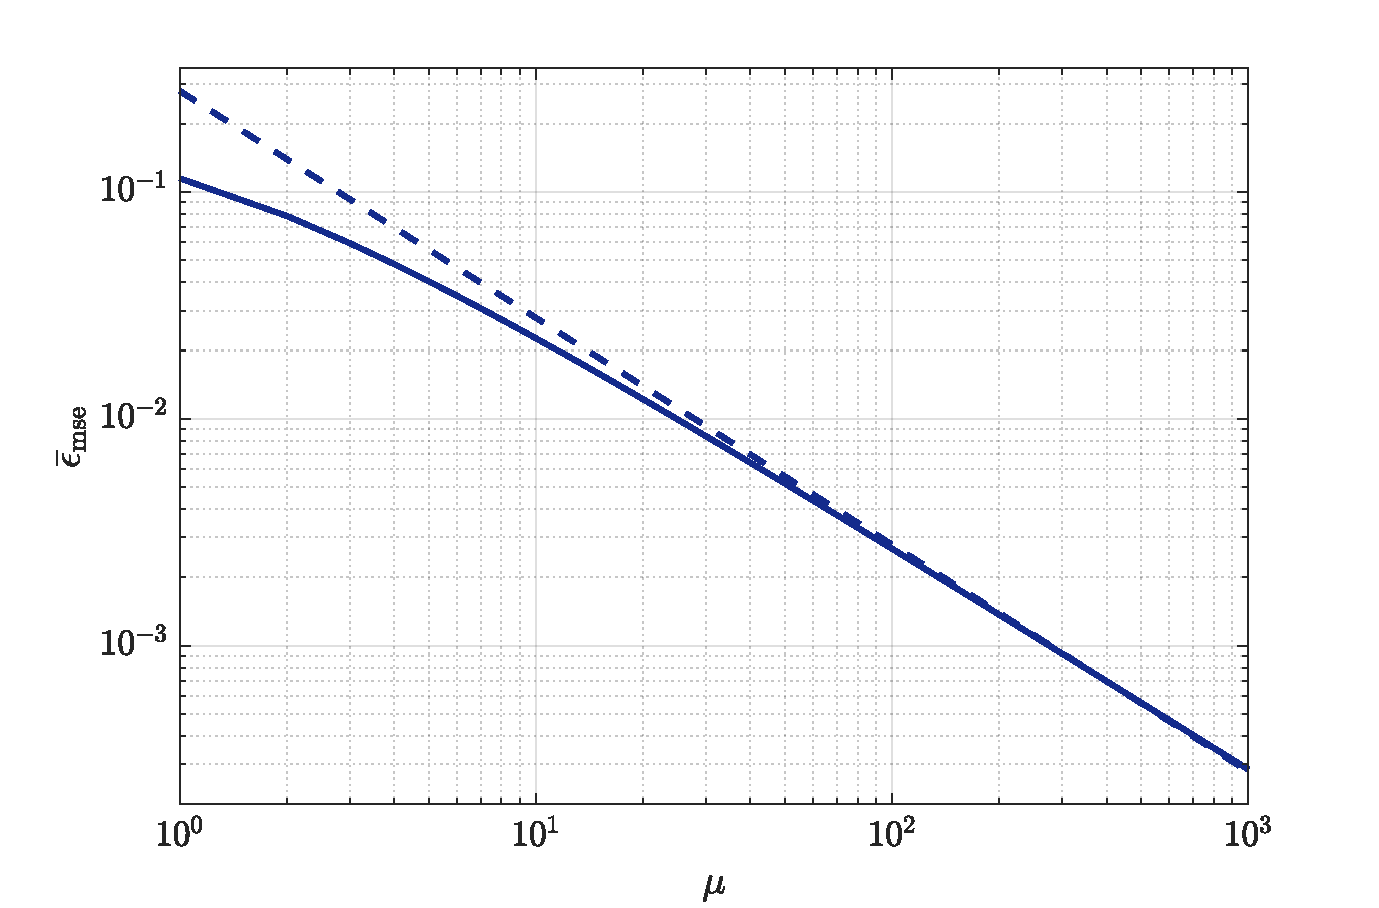
\includegraphics[trim={0.75cm 0.1cm 1.3cm 1cm},clip,width=14.75cm]{ch8_fig1}
	\caption[Shot-by-shot quantum bound with photon losses]{Mean square error based on the optimal single-shot strategy (solid line) and quantum Cram\'{e}r-Rao bound (dashed line) for a two-photon state whose Fisher information is optimal (see \cite{dorner2009}) that is fed to a Mach-Zehnder interferometer with photon losses in its first arm, with $\eta=0.9$, $\bar{\phi} = \pi/4$ and $W_0 = \pi/2$.}
\label{lossy_plot}
\end{figure}

The next step is to calculate the optimal single-shot strategy. Assuming that the prior $p(\phi)$ is a flat density of width $W_0 = \pi/2$ and centred around $\bar{\phi} = \pi/4$, we can calculate $\rho = \int d\phi p(\phi)\rho(\phi)$, $\bar{\rho} = \int d\phi p(\phi)\rho(\phi)\phi$ and insert the results into $S\rho + \rho S = 2\bar{\rho}$ to find the optimal quantum estimator
\begin{equation}
S=\frac{1}{76\pi}
\begin{pmatrix} 
19\pi^2 & 0 & 0 & 0 \\
0 & 19\pi^2 & 0 & -24 \sqrt{10} \\
0 & 0 & 19\pi^2 & 0 \\
0 & -24 \sqrt{10} & 0 & 19\pi^2
\end{pmatrix}.
\end{equation}
Using the eigenspaces of $S$ we may construct the projective measurement $\ket{s_1}=(-\ket{0,2}+\ket{2,0})/\sqrt{2}$, $\ket{s_2}=(\ket{0,2}+\ket{2,0})/\sqrt{2}$, $\ket{s_3}=\ket{1,0}$ and $\ket{s_4}=\ket{0,0}$. However, note that, in this case, the optimal single-shot POM is not unique due to the degeneracy of one of the eigenvalues of $S$.

Finally, we calculate the mean square error in equation (\ref{shotbyshotmse}) using this optimal single-shot measurement. The result has been represented in figure \ref{lossy_plot} as a solid line, which also includes the quantum Cram\'{e}r-Rao bound as a dashed line (the latter can be obtained using the expression for the Fisher information $F_q$ provided in \cite{dorner2009}). As we can see, the Bayesian error is very close to the quantum Cram\'{e}r-Rao bound, although a perfect convergence cannot be observed because the mean square error crosses the bound when $\mu \approx 4 \cdot 10^2$. 

It may be verified that the reason for this discrepancy is that the classical Fisher information associated with the chosen POM is no longer parameter-independent, and it only achieves the quantum Cram\'{e}r-Rao bound for certain values of $\phi$. As such, and recalling our discussion about the asymptotic regime in chapter \ref{chap:nonasymptotic}, this implies that, in this case, the true asymptotic approximation is $\int d\phi \hspace{0.15em}p(\phi)/[\mu F(\phi)]$, and not $1/(\mu F_q)$. Remarkably, this is unlike for the ideal schemes in chapter \ref{chap:limited}. Thus this phenomenon sets the scene for a future study about the fundamental limits that we may expect when the data is scarce and there is a certain amount of noise\footnote{We draw attention to the fact that the explanation for the discrepancy in figure \ref{lossy_plot} provided in this section complements the initial test with photon losses in our publication \cite{jesus2018}, where such explanation was not explicitly identified.}. 

On the other hand, if we were to look at this result from a more practical point of view, then we could conclude that a reasonable amount of photon losses does not alter substantially our findings for ideal schemes, since we have verified that after $\mu = 10^3$ repetitions the relative error between the Bayesian uncertainty and the quantum Cram\'{e}r-Rao bound in figure \ref{lossy_plot} is just $\varepsilon = 0.02$. Nevertheless, a deeper investigation including other sources of noise, new probe states and realistic measurements is required in order to construct a complete picture of the effect of noise when the available data is limited. 

\section{A more fundamental perspective}
\label{sec:fundtime}

While quantum metrology and quantum estimation theory are, in a sense, frameworks with an eminently pragmatic purpose, it is well known that they can also be used in a more fundamental way to construct uncertainty relations of a generalised type \cite{braunstein1996, helstrom1976}. In fact, we have already encountered a manifestation of this connection in section \ref{subsec:optint}, where we reviewed a path to arrive at the quantum Cram\'{e}r-Rao bound for pure states from a Mandelstam-Tamm uncertainty relation (see \cite{HofmannHolger2009}). 

Suppose we look at the quantum Cram\'{e}r-Rao bound as a generalised uncertainty relation. The results in this thesis have demonstrated the advantages of treating this bound as a limiting case of a more general theory, such that the former only emerges when certain conditions are fulfilled. If we follow this logic, then it is natural to enquire whether it would be possible to construct some sort of uncertainty relation that incorporates both the effect of the prior information and a finite number of shots. That a generalised uncertainty relation can be constructed with Bayesian quantities was in fact shown by Helstrom \cite{helstrom1976} using the sine error in equation (\ref{sinerror}) for a single shot, while Braunstein \emph{et al.} \cite{braunstein1996} considered several copies of the probe state within the context of the Cram\'{e}r-Rao bound. In view of this, by constructing an uncertainty relation that combines both features we would be able to extend the scope of uncertainty relations in quantum mechanics to cover scenarios where the data is limited and only a moderate amount of prior information is available. 

Although we leave for future work the detailed exploration of this possibility and of its potential consequences, we would like to illustrate what our non-asymptotic methodology has to say about this line of thought. To achieve that goal, let us consider a scenario where the parameter that we wish to estimate is the elapsed time from the evolution of a two-level system, which we denote by $t$. If the system is prepared in the pure state $\rho_0 = (\mathbb{I}+\sigma_x)/2$, the parameter is encoded as $\rho(t) = \mathrm{e}^{-i K t} \rho_0 \mathrm{e}^{i K t}$ and the generator is $K = (E/\hbar)\sigma_z$, with energy $E$, then the quantum Fisher information is
\begin{equation}
F_q = 4\left(\langle \psi_0 | K^2 | \psi_0 \rangle - \langle \psi_0 | K | \psi_0 \rangle^2\right) = 4\left[\mathrm{Tr}(\rho_0 K^2) -\mathrm{Tr}\left(\rho_0 K\right)^2\right] = \frac{4 E^2}{\hbar^2},
\end{equation}
so that the value of the quantum Cram\'{e}r-Rao bound is
\begin{equation}
\bar{\epsilon}_\mathrm{cr} = \frac{1}{\mu F_q} = \frac{\hbar^2}{4\mu E^2}.
\end{equation}
If we are working in the asymptotic regime, then $\bar{\epsilon}_{\mathrm{mse}}\gtrsim \bar{\epsilon}_{\mathrm{cr}}$, so that we can write 
\begin{equation}
E^2 \hspace{0.1em}\bar{\epsilon}_{\mathrm{mse}} \equiv E^2 \Delta t^2 \gtrsim \frac{\hbar^2}{4\mu},
\end{equation}
which indeed has the form that we would expect for an uncertainty relation.

To saturate this bound, first we need a measurement for which $F(t) = F_q$, where $F(t)$ is the classical Fisher information. We can verify by a direct calculation that a POM that satisfies such condition is $\ketbra{s_\pm} = (\mathbb{I} \pm \sigma_y)/2$. In particular, given that the transformed state is
\begin{align}
\rho(t) &= \mathrm{exp}\left(-i E t\sigma_z/\hbar\right)\rho_0\hspace{0.15em}\mathrm{exp}\left(i E t\sigma_z/\hbar\right)
\nonumber \\
&= \frac{1}{2}\left[\mathbb{I} + \mathrm{cos}\left(2 E t/\hbar\right)\sigma_x + \mathrm{sin}\left(2 E t/\hbar\right)\sigma_y\right],
\end{align}
where we have used the fact that $\mathrm{exp}(i A \sigma_z) = \mathrm{cos}(A)\mathbb{I} + i \mathrm{sin}(A)\sigma_z$, and that the single-shot likelihood function for the aforementioned POM is
\begin{equation}
p(s_\pm|t) = \langle s_\pm | \rho(t) | s_\pm \rangle = \frac{1}{2} \left[1 \pm \mathrm{sin}\left(2 E t/\hbar\right)\right],
\end{equation}
we find that
\begin{eqnarray}
F(t) = \frac{1}{p(s_{+}|t)}\left[\frac{\partial p(s_{+}|t)}{\partial t}\right]^2 + \frac{1}{p(s_{-}|t)}\left[\frac{\partial p(s_{-}|t)}{\partial t}\right]^2 = \frac{4 E^2}{\hbar^2} = F_q,
\end{eqnarray}
as desired. Furthermore, from our findings in chapter \ref{chap:nonasymptotic} we know that to reach the Cram\'{e}r-Rao bound we also need to select a region of the parameter domain where the likelihood does not contain ambiguous information. Assuming a flat prior in such region, we have seen that one way of identifying the intrinsic width\footnote{We recall that we have defined the intrinsic width as the largest width that a flat prior can have while the likelihood function still presents a unique absolute maximum after many repetitions (see chapter \ref{chap:nonasymptotic}).} $W_\mathrm{int}$ is to examine the maxima of the posterior probability $p(t|\boldsymbol{s}) \propto p(\boldsymbol{s}| t)$, where $\boldsymbol{s} = (s_1, \dots, s_\mu)$ are the outcomes of $\mu$ repetitions of the experiment. Figure \ref{timeestimation}.i shows the result of this operation, and upon its inspection we  conclude that $W_\mathrm{int} = \pi \hbar/(2E)$ if one of the boundaries of our prior probability is $(2k+1)\pi \hbar/(4E)$, where $k$ is an integer. The final requirement to achieve the Cram\'{e}r-Rao bound is to repeat the experiment a large number of times. 
 
\begin{figure}[t]
\centering
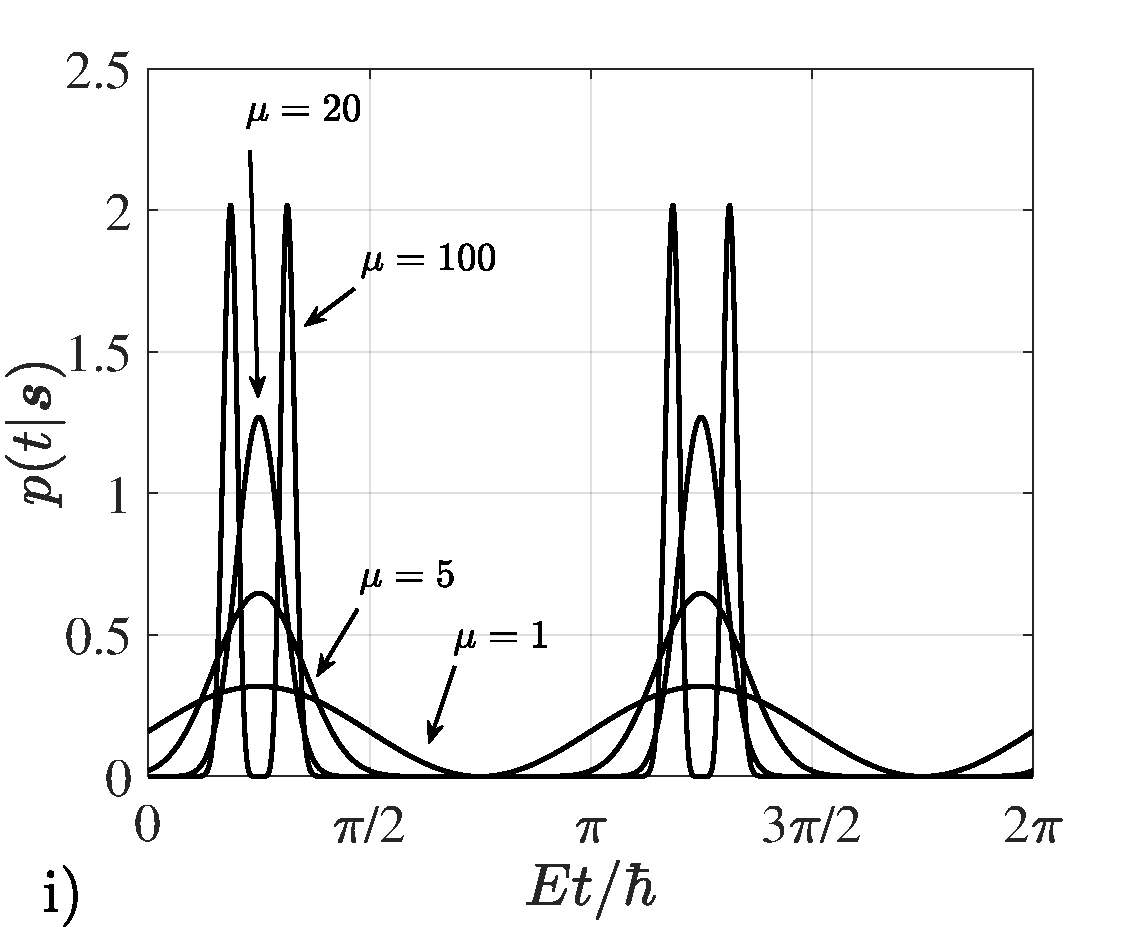
\includegraphics[trim={0.1cm 0.1cm 0.5cm 0.5cm},clip,width=7.7cm]{pictures/ch8_fig2i}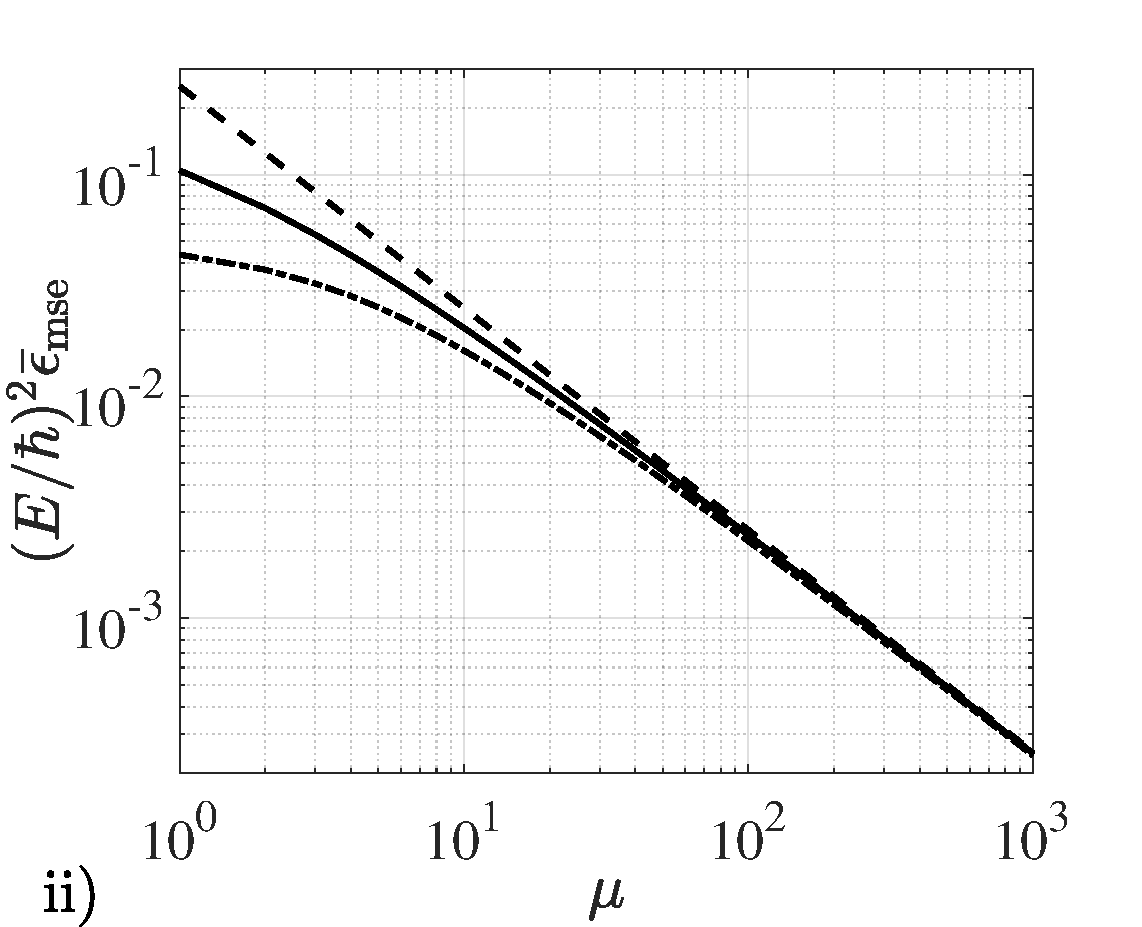
\includegraphics[trim={0cm 0cm 0.5cm 0.5cm},clip,width=7.7cm]{pictures/ch8_fig2ii} 
\caption[Bayesian time estimation]{i) Posterior probabilities for random simulations of 1, 5, 20 and 100 trials, a flat prior, the POM $\ketbra{s_\pm} = (\mathbb{I} \pm \sigma_y)/2$ and the state $\rho_0 = (\mathbb{I}+\sigma_x)/2$. In (ii) we have represented the mean square error for the previous configuration and prior widths $W_0=\pi\hbar/(2E)$ (solid line) and $W_0=\pi\hbar/(4E)$ (dash-dotted line), while the dashed line is the quantum Cram\'{e}r-Rao bound, which in this section plays the role of a generalised uncertainty relation. We draw attention to the fact that while the prior information alters the precision in the regime of limited data, both Bayesian schemes converge to the same asymptotic optimum.}
\label{timeestimation}
\end{figure}

We shall now compare this bound with our shot-by-shot method, which requires us to calculate the single-shot optimal POM. Suppose that we write our flat prior as\footnote{This form is more convenient to take into account the fact that the intrinsic width depends here on the origin of the prior.} $p(t) = 1/W_0$, for $t\in[a_0,a_0+W_0]$, and zero otherwise, where $a_0 = \pi\hbar/(4E)$ and $W_0 = W_{\mathrm{int}} = \pi\hbar/(2E)$. In that case, and recalling that the quantum estimator $S$ is given by $S\rho + \rho S = 2\bar{\rho}$, with $\rho = \int dt\hspace{0.15em} p(t)\rho(t)$ and $\bar{\rho} = \int dt\hspace{0.15em}p(t)\rho(t)t$, we find that 
\begin{equation}
S = \frac{\pi\hbar}{2E} \left(\mathbb{I}-\frac{2\sigma_y}{\pi^2}\right).
\end{equation}
The projectors of this operator are precisely the POM elements that we have examined in the previous paragraph, that is, $\ketbra{s_\pm} = (\mathbb{I} \pm \sigma_y)/2$. Hence, for this arrangement we have that the same measurement scheme that is optimal asymptotically is also optimal for a single-shot. Adapting the shot-by-shot uncertainty in section \ref{subsec:shotbyshot} to our present case we conclude that the error to be calculated is 
\begin{equation}
\bar{\epsilon}_{\mathrm{mse}} = \int d\boldsymbol{s}~p(\boldsymbol{s}) \left\lbrace \int dt\hspace{0.15em}p(t|\boldsymbol{s}) t^2 - \left[\int dt\hspace{0.15em} p(t|\boldsymbol{s}) t \right]^2 \right\rbrace,
\label{errortime}
\end{equation}
where the posterior is $p(t|\boldsymbol{s})= p(t) p(\boldsymbol{s}|t)/p(\boldsymbol{s})$, the likelihood for $\mu$ trials is $p(\boldsymbol{s}|t) = \prod_{i=1}^\mu \langle s_i | \rho(t) |s_i \rangle$ and $p(\boldsymbol{s}) = \int dt \hspace{0.15em}p(t)p(\boldsymbol{s}|t)$. 

The result of the previous calculation has been represented as the solid line of figure \ref{timeestimation}.ii, while the quantum Cram\'{e}r-Rao bound is the dashed line. As we can see, the asymptotic bound underestimates the precision when the number of repetitions is low, since our shot-by-shot uncertainty is lower in such regime. The reason for this discrepancy is that the latter is taking into account a certain amount of prior information, which is consistent with the qualitative picture that our results in previous chapters have revealed. The novelty here is that we are looking at the quantum Cram\'{e}r-Rao bound as a generalised uncertainty relation. Since the prior knowledge that goes into the mean square error is precisely taking into account the requirements to saturate the Cram\'{e}r-Rao bound, one way of interpreting this result is to conclude that an uncertainty relation that does not include the combined effect of the prior information and a finite number of trials might be losing important information about the fundamental limits of the scheme under analysis. This conjecture, should it be confirmed, might have important consequences for our basic understanding of uncertainty relations.  

\section{Summary of results and conclusions}

Our non-asymptotic methodology promises to open new and exciting lines of future research. On the practical side, the next natural step is to include the effect of noise within our formalism, and a first initial test of this possibility has been carried out using a lossy interferometer. This calculation has revealed that while our method may be applied to such scenario, there are also important differences with respect to the ideal case. Regarding the technical limitations that we have found for the numerical calculation of Bayesian quantities, we have identified the extension of our algorithms to cases with $d\geqslant 3 $ natural parameters as a key step, so that we can keep exploring the interesting interplay that we have uncovered between correlations and a limited amount of data. Finally, we have explored the possibility of using our methodology in a more fundamental context, and we have conjectured the potential existence of generalised uncertainty relations that include the combined effect of a limited amount of data and a moderate prior knowledge, illustrating this idea by applying our shot-by-shot method to the problem of estimating the elapsed time from the evolution of a quantum system. 